\documentclass[a4paper, 12pt, fleqn]{article}

\usepackage{amsmath}
\usepackage{amsthm}
\usepackage{amssymb}
\usepackage[margin=1in]{geometry}
\usepackage{xcolor}
\usepackage{float}
\usepackage{url}
\usepackage{array}
\usepackage{comment}
\usepackage[bookmarksnumbered=true,hypertexnames=false]{hyperref}
\usepackage{algorithm, algpseudocode}
\usepackage[capitalize,sort]{cleveref}

\hypersetup{
    colorlinks,
    linkcolor={red!50!black},
    citecolor={red!50!black},
    urlcolor={blue!50!black}
}

% THEOREMS

\newtheorem{theorem}{Theorem}
\newtheorem{definition}{Definition}
\newtheorem{example}{Example}
\newtheorem{corollary}{Corollary}[theorem]
\newtheorem{lemma}[theorem]{Lemma}

% SHORTHANDS

\newcommand*{\Th}{^{\textrm{th}}}
\newcommand*{\WLoG}{Without loss of generality}
\newcommand*{\wLoG}{without loss of generality}
\newcommand*{\wrt}{with respect to}

% SYMBOLS

\let\eps\epsilon
\newcommand*{\defeq}{:=}

% MATH

\newcommand*{\floor}[1]{\left\lfloor #1 \right\rfloor}
\newcommand*{\smallfloor}[1]{\lfloor #1 \rfloor}
\newcommand*{\ceil}[1]{\left\lceil #1 \right\rceil}
\newcommand*{\smallceil}[1]{\lceil #1 \rceil}
\newcommand*{\abs}[1]{\left\lvert #1 \right\rvert}
\newcommand*{\smallabs}[1]{\lvert #1 \rvert}
\newcommand*{\norm}[1]{\left\lVert #1 \right\rVert}
\newcommand*{\smallnorm}[1]{\lVert #1 \rVert}
\newcommand*{\Z}{\mathbb{Z}}
\DeclareMathOperator*{\E}{E}
\DeclareMathOperator*{\Var}{Var}
\DeclareMathOperator*{\argmin}{argmin}
\DeclareMathOperator*{\argmax}{argmax}
\DeclareMathOperator{\poly}{poly}
\DeclareMathOperator{\opt}{opt}
\newcommand*{\OPT}{\mathrm{OPT}}

% INITIALIZATIONS

\newcommand{\initMinimal}{
\setlength{\parindent}{0pt}
\setlength{\parskip}{0.5em}
}
\newcommand{\initFromContents}{
\tableofcontents
\newpage
\initMinimal{}
}
\newcommand{\initAfterBeginDocument}{
\maketitle
\initFromContents{}
}
\newcommand{\addMyBib}{
\bibliographystyle{plainurl}
\bibliography{bibdb}
}

\author{Eklavya Sharma}
\date{\empty}

\usepackage{diagbox}
\usepackage{tikz}
\usetikzlibrary{arrows.meta}

%\pagecolor[HTML]{fbf0da}
%\color[HTML]{433423}

\title{Strategic Form Games}

\begin{document}

\maketitle
\initMinimal{}

Game Theory is the study of mathematical models of interaction
between rational and intelligent decision makers
(the decision makers are also called \emph{agents} or \emph{players}).
We will look at one such model here, called \emph{strategic form games}.

A strategic form game $\Gamma$ is a tuple
$(N, (S_1, S_2, \ldots, S_n), (u_1, u_2, \ldots, u_n))$, where
\begin{itemize}
\item $N \defeq \{1, 2, \ldots, n\}$ is called the set of players.
\item For each $i \in N$, $S_i$ is called the \emph{strategy set} of player $i$.
    Each element in $S_i$ is called a \emph{strategy} or \emph{action}.
\item $S \defeq S_1 \times S_2 \times \ldots \times S_n$ is called the
    \emph{strategy profile collection} or \emph{outcome set}.
    Each element of $S$ is the tuple $s \defeq (s_1, s_2, \ldots, s_n)$,
    called a \emph{strategy profile} or \emph{outcome}.
    Here $s_i$ corresponds to the action of player $i$.
\item $u_i: S \mapsto \mathbb{R}$ is called the utility function of player $i$.
\end{itemize}

We will usually use a more concise notation for vectors of length $n$, for example,\\
$(S_1, S_2, \ldots, S_n) \defeq (S_i)_{i \in N}$
and $(u_1, u_2, \ldots, u_n) \defeq (u_i)_{i \in N}$.

In this model, each player $i$ will simultaneously choose an action $s_i \in S_i$,
and will receive utility $u_i(s)$, where $s \defeq (s_i)_{i \in N}$.
The players cannot coordinate, i.e., they choose their actions independently.
Our aim in game theory is to predict the outcome $s$ of the game
under the following assumptions:
\begin{itemize}
\item Rationality: each player $i$ wishes to maximize her utility $u_i(s)$.
\item Intelligence: all players are extremely skilled (at game theory, math, logic, etc.)
    and resourceful.
\item Common knowledge: all players know $\Gamma$
    (i.e., they know the number of players, the strategy sets of all players
    and the utility functions of all players), they know that all players know $\Gamma$,
    they know that all players know that all players know $\Gamma$, and so on.
\end{itemize}

For a strategy profile $s$, let $s_{-i} \defeq (s_1, s_2, \ldots, s_{i-1}, s_{i+1}, \ldots, s_n)$.
Let $S_{-i} \defeq S_1 \times S_2 \times \ldots \times S_{i-1} \times S_{i+1} \times \ldots \times S_n$.

\section{Examples}

\subsection{Coordination game}

There are 2 players: $1$ and $2$. There are 2 locations: $A$ and $B$.
Each player has to choose a location. The players want to spend time together,
so if they choose different locations, their utility is 0.
They both like place $A$ more than place $B$,
so if both choose $A$, they both have utility 100,
and if both choose $B$, they both have utility 10.

To model this situation as a strategic form game
$(N, (S_i)_{i \in N}, (u_i)_{i \in N})$ we have
\begin{itemize}
\item $N = \{1, 2\}$.
\item $S_1 = S_2 = \{A, B\}$.
\item For each $i \in N$, ${\displaystyle u_i((s_1, s_2)) = \begin{cases}
0 & s_1 \neq s_2
\\ 100 & s_1 = s_2 = A
\\ 10 & s_1 = s_2 = B
\end{cases}}$.
\end{itemize}
We can depict $(u_1, u_2)$ as a matrix, called the \emph{payoff matrix}:
\begin{center}
\begin{tabular}{|c|c|c|}
\hline
\diagbox{1}{2} & A & B
\\ \hline
A & 100, 100 & 0, 0
\\ \hline
B & 0, 0 & 10, 10
\\ \hline
\end{tabular}
\end{center}

\subsection{Braess Paradox}

Consider the following road network, where 1000 players wish to travel from $S$ to $T$,
and each player wants to minimize the time taken to travel from $S$ to $T$.

\begin{center}
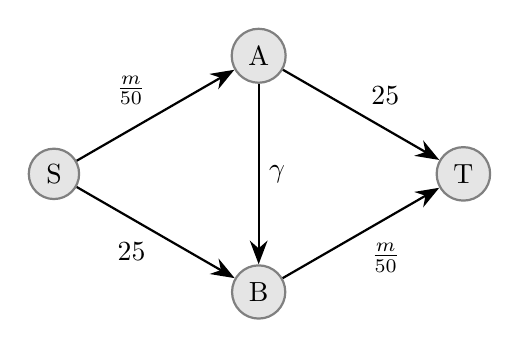
\begin{tikzpicture}[vertex/.style={circle,fill=black!10,draw=black!50,thick},
myedge/.style={-{Stealth[length=3mm]},thick},scale=1.0]
\node[vertex] (B) at (0, -1.5) {B};
\node[vertex] (A) at (0,  1.5) {A};
\node[vertex] (S) at (-2.6, 0) {S};
\node[vertex] (T) at ( 2.6, 0) {T};
\draw[myedge] (S) -- node[anchor=south east] {$\frac{m}{50}$} (A);
\draw[myedge] (A) -- node[anchor=south west] {$25$} (T);
\draw[myedge] (S) -- node[anchor=north east] {$25$} (B);
\draw[myedge] (B) -- node[anchor=north west] {$\frac{m}{50}$} (T);
\draw[myedge] (A) -- node[anchor=west] {$\gamma$} (B);
\end{tikzpicture}
\end{center}

The weight of an edge gives the time taken to traverse that edge.
Here $m$ is the number of vehicles using that road, and $\gamma$ is a constant.
The utility of a player is the negative of the time taken to travel from $S$ to $T$.

Each player has 3 strategies:
\begin{itemize}
\item Strategy $A$: go from $S$ to $A$ to $T$.
\item Strategy $B$: go from $S$ to $B$ to $T$.
\item Strategy $AB$: go from $S$ to $A$ to $B$ to $T$.
\end{itemize}
For a strategy profile $s$ and action $X$,
let $n_X(s)$ be the number of players who chose strategy $X$.
Note that $n_A(s) + n_B(s) + n_{AB}(s) = 1000$.
We can define the strategic form game $(N, (S_i)_{i \in N}, (u_i)_{i \in N})$ as follows:

\begin{itemize}
\item $N = \{1, 2, \ldots, 1000\}$.
\item For each $i \in N$, $S_i = \{A, B, AB\}$.
\item For each $i \in N$, ${\displaystyle u_i(s) = -\begin{cases}
\displaystyle \frac{n_A(s) + n_{AB}(s)}{50} + 25 & s_i = A
\\[10pt] \displaystyle 25 + \frac{n_B(s) + n_{AB}(s)}{50} & s_i = B
\\[10pt] \displaystyle 20 + \gamma + \frac{n_{AB}(s)}{50} & s_i = AB
\end{cases}}$.
\end{itemize}

There are two important values of $\gamma$ that we will consider: $0$ and $\infty$.
Intuitively, it looks like congestion should be lower for the $\gamma = 0$ case,
but we will later see that congestion is actually lower for the $\gamma = \infty$.

\subsection{Sealed bid auction}

An item is being sold at an auction.
There are $n$ bidders who participate in the auction, numbered from 1 to $n$.
Each bidder has a valuation $v_i$ for the item, which is not known to other players.

Each player $i$ simultaneously places a bid of $s_i \in \mathbb{R}$ for the item.
$s \defeq (s_1, s_2, \ldots, s_n)$ is called the \emph{bid profile}.
The winner is the player with the highest bid.
If there are multiple players with the highest bid,
then the player among them with the lowest index is the winner.
Let $w$ be the winning player. Player $w$ will pay $t(s)$ for the item
($t$ is a function of the bid profile $s$).
Other players don't pay anything.
The utility of player $w$ is $v_w - t(s)$. The utility of other players is $0$.

We can model this as a strategic form game $(N, (S_i)_{i \in N}, (u_i)_{i \in N})$ as follows:
\begin{itemize}
\item $N = \{1, 2, \ldots, n\}$.
\item For each $i \in N$, $S_i = \mathbb{R}$.
\item For each $i \in N$, $u_i(s) = \begin{cases}
\displaystyle v_i - t(s) & \textrm{ if player $i$ wins}
\\ \displaystyle 0 & \textrm{ otherwise}
\end{cases}$.
\end{itemize}

%\addMyBib{}

\end{document}
